\section{Results and Discussion}

% TODO: RnD
Due to the nature of the experimentation, there are five versions each implemented machine learning model, each with different hyperparameters. However, for the interpretation and discussion of results, only the best performing model are taken into consideration. 

\subsection{Logistic Regression results}

Due to the polynomial features, there were 465 columns fed into the models, because of this, it's best to instead take note of the most significant coefficients from the model. Looking at table \ref{tab:lr top5 coef}, it can be observed that the most significant features are all interaction features.

\begin{table}[H]
    \caption{Top 5 Features in the logistic regression model}
    \label{tab:lr top5 coef}
    \begin{tabularx}{\linewidth}{l>{\centering\arraybackslash}X}
        \toprule
        Feature & Value \\
        \midrule
        MntFruits \\ A\_Marital\_Status\_Single\_Kidhome & 0.979750 \\
        \midrule
        MntMeatProducts \\ A\_Marital\_Status\_Married\_Teenhome & 0.952025 \\
        \midrule
        MntWines \\ A\_Marital\_Status\_Together\_Teenhome & 0.844306 \\
        \midrule
        Education\_Master \\ A\_Marital\_Status\_Single\_Kidhome & 0.814164 \\
        \midrule
        MntWines \\ NumWebPurchases & 0.763514 \\
        \bottomrule
    \end{tabularx}
\end{table}

It is observed that people who bought fruits and are married with a kid at home are very likely to respond and accept the offer. The likeliness to accept the offer can also be seen with married people with a teen at home who also bought meat products in the last two years, people that live with someone (\texttt{Together} marital status value) that buys wines with a teen at home, single people who achieved masters education with a kid at home, as well as people who bought wines in the last two years that also bought products at the company's website.

\subsection{SVM}

Since the best model tested in the SVC models is a linear model, it can be interpreted that the coefficients to understand how the model has learned. Table \ref{tab:svm top5 coef} shows a lot of similarity with the top five coefficients of the linear regression model. 

\begin{table}[H]
    \caption{Top 5 features in the SVM model}
    \label{tab:svm top5 coef}
    \begin{tabularx}{\linewidth}{l>{\centering\arraybackslash}X}
        \toprule
        Feature & Value \\
        \midrule
        MntWines NumWebPurchases & 0.904773 \\
        A\_Marital\_Status\_Married\_Kidhome \\ A\_Marital\_Status\_Married\_Teenhome & 0.804857 \\
        MntFruits \\ A\_Marital\_Status\_Single\_Kidhome & 0.803837 \\
        NumWebVisitsMonth \\ A\_Marital\_Status\_Single\_Kidhome & 0.769760 \\
        Recency \\ Days\_Since\_Customer & 0.733147 \\
        \bottomrule
    \end{tabularx}
\end{table}

As it turns out, the support vector machine model's top five coefficients has two features similar to the top five of the linear regression model. This would make sense because although they are different machine learning models, grid search algorithm has decided that the best hyperparameters for the SVM included that the svm should use a linear kernel. This would imply that the data is much akin to being linearly separable. Table \ref{tab:svm top5 coef} implies the same ideas as it did for the features that were also in table \ref{tab:lr top5 coef}. For the features unique to table \ref{tab:svm top5 coef}, they simply imply that people who are married with children and teenagers at home, single with a kid at home that visits the company's website in the past month, and people who haven't bought in a while (high \texttt{Recency} value) that are also long standing customers (high \texttt{Days\_Since\_Customer} value) are more willing to respond and accept the offer.

It is a bit difficult to interpret the support vectors found by the SVM. Mainly because any aggregation to these found support vectors are only slightly different to the aggregations found in the original dataset. For example, the average \texttt{Year\_Birth} for the dataset is 1970.325371 while the average for the support vectors is 1970.030303; this is reflected to the other attributes even with different aggregation methods, whether it is the average, standard deviation, etc. the results only vary by a few units. This could be explained by the idea that maybe much of the data points are closer to decision boundary than expected. According to the model there are a total of 198 support vectors found in the dataset; 131 for no responses, and 67 for the responses. To put into perspective, out of the total 971 entries in the training set, 131 are support vectors, that is about 20.3\% of the training set. 

\subsection{Naive Bayes}

According to the implemented Bernoulli Naive Bayes, the log probability of a 0 response (not accepted) is -0.09726884, while a 1 response (accepted the offer) is -2.3785168. This means that the chance of accepting the offer is much lower in probability compared to rejecting it which would make sense given there is a heavy imbalance in the dataset where 1101 responses are 0 while only 113 entries have a response of 1.

When analyzing the log probability of a feature, the values imply the probability of a feature for a given class, i.e. $P(x_i \mid y)$. Just like the analysis of coefficients at the logistic regression and SVM models, there is too much features to be able to show them all. So, just as before, it is best to just look at the highest scoring (or alternatively, the lowest scoring) of the feature log probabilities.

\begin{table}[H]
    \caption{Top five highest feature probabilities for response 0}
    \label{tab:nb top5 0}
    \begin{tabularx}{\linewidth}{l>{\centering\arraybackslash}X}
        \toprule
        Feature & $Log P(x_i \mid y=0)$ \\
        \midrule
        Year\_Birth & -0.624380 \\
        \midrule
        Year\_Birth Recency & -0.641402 \\
        \midrule
        NumCatalogPurchases \\ Days\_Since\_Customer & -0.650023 \\
        \midrule
        NumCatalogPurchases & -0.650023 \\
        \midrule
        Recency & -0.650023 \\
        \bottomrule
    \end{tabularx}
\end{table}

\begin{table}[H]
    \caption{Top five highest feature probabilities for response 1}
    \label{tab:nb top5 1}
    \begin{tabularx}{\linewidth}{l>{\centering\arraybackslash}X}
    \toprule
     & 1 \\
    \midrule
    NumWebVisitsMonth \\ Days\_Since\_Customer & -0.148846 \\
    \midrule
    NumCatalogPurchases & -0.239230 \\
    \midrule
    Year\_Birth \\ NumCatalogPurchases & -0.239230 \\
    \midrule
    NumCatalogPurchases \\ Days\_Since\_Customer & -0.239230 \\
    \midrule
    NumCatalogPurchases \\ NumWebVisitsMonth & -0.252835 \\
    \bottomrule
    \end{tabularx}
\end{table}

Table \ref{tab:nb top5 0} shows that someones year of birth and combined it with the recency of purchases, as well as the amount of catalog purchases with their length as a customer, it determines that they will likely not accept. Note however that these are continuous variables, hence these probabilities behave more like distributions. On the other hand, for people who did respond, their visits at the website combined with their days as a customer, as well as their catalog purchases which can be combined with their year of birth days as a customer and visits at the website last month determine if they will accept the offer (see table \ref{tab:nb top5 1})

\subsection{Decision Trees}

\begin{figure}[H]
    \centering
    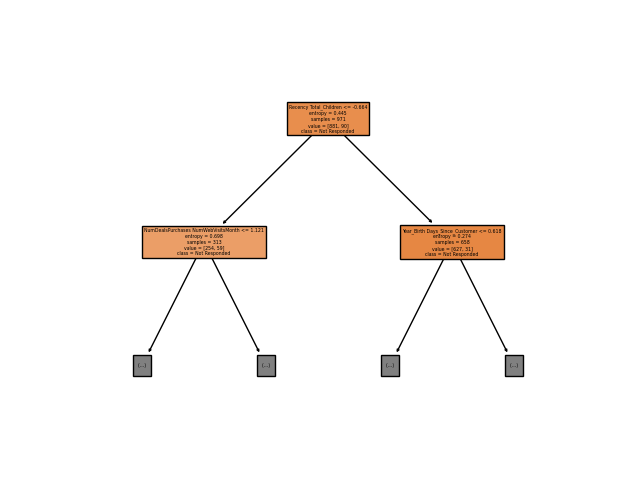
\includegraphics[width=\linewidth]{figures/decision_tree.png}
    \caption{Illustration of Decision Tree}
    \label{fig:tts cv}
\end{figure}

In the decision tree, the root node splits on the feature of \texttt{Recency Total_Children <= -0.664}. This indicates that the combination of these features is important in predicting the target variable, and uses the value of -0.664 as a threshold to give a two possible outcomes, considering that the features were standardized during preprocessing. If the condition is less than or equal to -0.664, then the left branch is taken; otherwise the right branch is taken. It implies that recency and number of children in the household are signifcanty factors in predicting customer response. 

Moreover, the left child node, \textt{NumDealsPurchases NumWebVisitsMonth <= 1.121}, and right child node, \textt{Year_Birth Days_Since_Customer <= 0.818} further splits the data to represent more classes to predict the value of target variable. These child nodes highlight the importance of the number of deals and website visits, and the customer's age and days since they first became a customer in predicting their response.

\subsection{K-Nearest Neighbor}
